\subsection{beamconf Struct Reference}
\label{structbeamconf}\index{beamconf@{beamconf}}
{\tt \#include $<$bpm\_\-interface.h$>$}

Collaboration diagram for beamconf:\nopagebreak
\begin{figure}[H]
\begin{center}
\leavevmode
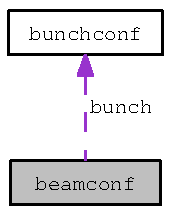
\includegraphics[width=59pt]{structbeamconf__coll__graph}
\end{center}
\end{figure}


\subsubsection{Detailed Description}
This structure contains the global beam parameters as well as a pointer to the array of bunches 

Definition at line 227 of file bpm\_\-interface.h.\subsubsection*{Data Fields}
\begin{CompactItemize}
\item 
int {\bf train\_\-num}
\item 
double {\bf beamrate}
\item 
double {\bf bunchrate}
\item 
int {\bf nbunches}
\item 
{\bf bunchconf\_\-t} $\ast$ {\bf bunch}
\item 
double {\bf position} [2]
\item 
double {\bf positionsigma} [2]
\item 
double {\bf slope} [2]
\item 
double {\bf slopesigma} [2]
\item 
double {\bf tilt} [2]
\item 
double {\bf tiltsigma} [2]
\item 
double {\bf bunchlength}
\item 
double {\bf bunchlengthsigma}
\item 
double {\bf energy}
\item 
double {\bf energysigma}
\item 
double {\bf charge}
\item 
double {\bf chargesigma}
\end{CompactItemize}


\subsubsection{Field Documentation}
\index{beamconf@{beamconf}!train\_\-num@{train\_\-num}}
\index{train\_\-num@{train\_\-num}!beamconf@{beamconf}}
\paragraph[train\_\-num]{\setlength{\rightskip}{0pt plus 5cm}int {\bf beamconf::train\_\-num}}\hfill\label{structbeamconf_f25a9f8d65fa4f04f9050414e0dcf891}


seq number of the train (evt num) 

Definition at line 228 of file bpm\_\-interface.h.\index{beamconf@{beamconf}!beamrate@{beamrate}}
\index{beamrate@{beamrate}!beamconf@{beamconf}}
\paragraph[beamrate]{\setlength{\rightskip}{0pt plus 5cm}double {\bf beamconf::beamrate}}\hfill\label{structbeamconf_9452259b166a06292909dd94e87bf9ae}


beam repetition rate (train to train) 

Definition at line 230 of file bpm\_\-interface.h.\index{beamconf@{beamconf}!bunchrate@{bunchrate}}
\index{bunchrate@{bunchrate}!beamconf@{beamconf}}
\paragraph[bunchrate]{\setlength{\rightskip}{0pt plus 5cm}double {\bf beamconf::bunchrate}}\hfill\label{structbeamconf_21abb80770607c1d48fef708c5dc4ebd}


bunch repetition rate (in the train) 

Definition at line 231 of file bpm\_\-interface.h.\index{beamconf@{beamconf}!nbunches@{nbunches}}
\index{nbunches@{nbunches}!beamconf@{beamconf}}
\paragraph[nbunches]{\setlength{\rightskip}{0pt plus 5cm}int {\bf beamconf::nbunches}}\hfill\label{structbeamconf_3957367666e4d2132d8a662941276f3a}


number of bunches per train 

Definition at line 232 of file bpm\_\-interface.h.

Referenced by generate\_\-bpmsignal(), and get\_\-bpmhits().\index{beamconf@{beamconf}!bunch@{bunch}}
\index{bunch@{bunch}!beamconf@{beamconf}}
\paragraph[bunch]{\setlength{\rightskip}{0pt plus 5cm}{\bf bunchconf\_\-t}$\ast$ {\bf beamconf::bunch}}\hfill\label{structbeamconf_9ded2879131ef6960f2c63893353c885}


list of pointers to the bunch conf structures 

Definition at line 234 of file bpm\_\-interface.h.

Referenced by generate\_\-bpmsignal(), and get\_\-bpmhits().\index{beamconf@{beamconf}!position@{position}}
\index{position@{position}!beamconf@{beamconf}}
\paragraph[position]{\setlength{\rightskip}{0pt plus 5cm}double {\bf beamconf::position}[2]}\hfill\label{structbeamconf_26b00990a201ad20363ff2affe6792fa}


beam position at the origin 

Definition at line 236 of file bpm\_\-interface.h.\index{beamconf@{beamconf}!positionsigma@{positionsigma}}
\index{positionsigma@{positionsigma}!beamconf@{beamconf}}
\paragraph[positionsigma]{\setlength{\rightskip}{0pt plus 5cm}double {\bf beamconf::positionsigma}[2]}\hfill\label{structbeamconf_3fd6fab4b89235e0a27d3733676f8eca}


position spread at the origin 

Definition at line 237 of file bpm\_\-interface.h.\index{beamconf@{beamconf}!slope@{slope}}
\index{slope@{slope}!beamconf@{beamconf}}
\paragraph[slope]{\setlength{\rightskip}{0pt plus 5cm}double {\bf beamconf::slope}[2]}\hfill\label{structbeamconf_71c30c68495a26878183645035cb8677}


beam slope at the origin 

Definition at line 239 of file bpm\_\-interface.h.\index{beamconf@{beamconf}!slopesigma@{slopesigma}}
\index{slopesigma@{slopesigma}!beamconf@{beamconf}}
\paragraph[slopesigma]{\setlength{\rightskip}{0pt plus 5cm}double {\bf beamconf::slopesigma}[2]}\hfill\label{structbeamconf_40ab197475399c5bb01b5abe25dee3d9}


slope spread at the origin 

Definition at line 240 of file bpm\_\-interface.h.\index{beamconf@{beamconf}!tilt@{tilt}}
\index{tilt@{tilt}!beamconf@{beamconf}}
\paragraph[tilt]{\setlength{\rightskip}{0pt plus 5cm}double {\bf beamconf::tilt}[2]}\hfill\label{structbeamconf_7465dd8acdcfce91e185a075334e2300}


bunch tilt at the origin 

Definition at line 242 of file bpm\_\-interface.h.\index{beamconf@{beamconf}!tiltsigma@{tiltsigma}}
\index{tiltsigma@{tiltsigma}!beamconf@{beamconf}}
\paragraph[tiltsigma]{\setlength{\rightskip}{0pt plus 5cm}double {\bf beamconf::tiltsigma}[2]}\hfill\label{structbeamconf_64040fb7876b2b4b8969154ab4aa387d}


tilt spread at the origin 

Definition at line 243 of file bpm\_\-interface.h.\index{beamconf@{beamconf}!bunchlength@{bunchlength}}
\index{bunchlength@{bunchlength}!beamconf@{beamconf}}
\paragraph[bunchlength]{\setlength{\rightskip}{0pt plus 5cm}double {\bf beamconf::bunchlength}}\hfill\label{structbeamconf_77503373031b8d15c31f697e8b8f5257}


bunch length at the origin 

Definition at line 245 of file bpm\_\-interface.h.\index{beamconf@{beamconf}!bunchlengthsigma@{bunchlengthsigma}}
\index{bunchlengthsigma@{bunchlengthsigma}!beamconf@{beamconf}}
\paragraph[bunchlengthsigma]{\setlength{\rightskip}{0pt plus 5cm}double {\bf beamconf::bunchlengthsigma}}\hfill\label{structbeamconf_166c8fdd8f3720c15faa4ba77b234d2c}


length spread at the origin 

Definition at line 246 of file bpm\_\-interface.h.\index{beamconf@{beamconf}!energy@{energy}}
\index{energy@{energy}!beamconf@{beamconf}}
\paragraph[energy]{\setlength{\rightskip}{0pt plus 5cm}double {\bf beamconf::energy}}\hfill\label{structbeamconf_259020346afa58ec8360e5098e8d9ab4}


beam energy (in GeV) at the origin 

Definition at line 248 of file bpm\_\-interface.h.\index{beamconf@{beamconf}!energysigma@{energysigma}}
\index{energysigma@{energysigma}!beamconf@{beamconf}}
\paragraph[energysigma]{\setlength{\rightskip}{0pt plus 5cm}double {\bf beamconf::energysigma}}\hfill\label{structbeamconf_3a7e535010155e32742b08a4a7b68415}


beam energy spread 

Definition at line 249 of file bpm\_\-interface.h.\index{beamconf@{beamconf}!charge@{charge}}
\index{charge@{charge}!beamconf@{beamconf}}
\paragraph[charge]{\setlength{\rightskip}{0pt plus 5cm}double {\bf beamconf::charge}}\hfill\label{structbeamconf_c06ea1a62a94875a08d0ff3ffeed5b18}


bunch charge (in nC) 

Definition at line 250 of file bpm\_\-interface.h.\index{beamconf@{beamconf}!chargesigma@{chargesigma}}
\index{chargesigma@{chargesigma}!beamconf@{beamconf}}
\paragraph[chargesigma]{\setlength{\rightskip}{0pt plus 5cm}double {\bf beamconf::chargesigma}}\hfill\label{structbeamconf_2bd344a9266ed88379a987c5a845f986}


charge spread 

Definition at line 251 of file bpm\_\-interface.h.

The documentation for this struct was generated from the following file:\begin{CompactItemize}
\item 
bpminterface/{\bf bpm\_\-interface.h}\end{CompactItemize}
